\documentclass[12pt, oneside]{article}

\usepackage[a4paper, total={6in, 8in}]{geometry}
\usepackage{amssymb}
\usepackage{tikz}
\usetikzlibrary{calc}

\begin{document}

\title{Model Inference from Protein Time-Course in Hematopoietic Stem Cells}

\date{\today}

\author{Pandu Raharja \and Rene Schoeffel}

\maketitle

\begin{abstract}
Stochasticity of gene expression becomes apparent when studying the dynamics of single cells rather tan a population of cells. These fluctuations in gene expression in fact reveal more information about the underlying mechanisms of transcription and translation than one could obtain from population averages.

In this paper we developed a particle filtering algorithm to infer the parameters of stochastic models from single cell time series data. In particular, we apply this method to time-lapse microscopy data of two transcription factors (\texttt{Pu.1} and \texttt{Gata.1}) in blood stem cells. These transcription are thought to play a major role in stem cell differentiation.

Our results provided several insights into the dynamics of blood stem cells maturation and specifically in the single ell environment, we managed to gain several valuable insigts on the dynamics of the interaction between two transcription factors on the outcome of cell maturation.
\end{abstract}

\section{Introduction}

\section{Experimental Setting}

The cells were put in a culture for one week. A video of the cells would then be taken for the whole duration of one week. An automatic detection program tracks down each cell uniquely within the video frame and every 20-30 minutes, protein expression levels of each cell would then be measured. The expressed protein of interests (in our case \texttt{Pu.1} and \texttt{Gata.1}) were hybridized with distinct fluorescence proteins, which would allow for the expression level measurement at each time point.

\section{Models}

\subsection{Particle Filtering}

\subsubsection{Particle}

We use particle filtering in our simulation. Particle filtering is a family of methods that use utilize the concept of \textit{particle}. A particle $\mathcal{K}$ is defined as a triple of trajectory $X$, parameter set $\theta$ and assumed model $\mathcal{M}$,

$$
\mathcal{K} := (X, \theta, \mathcal{M})
$$

Note that a trajectory is different from the experimental data $\mathcal{D}$. A trajectory is the result of the simulation done by applying the parameters onto our model. In functional notation we would assume the i-th value of the trajectory $X_i$ to be a function of the i-th value of the trajectory, the model and the parameters,

$$
X_i = f(X_{i - 1}, \mathcal{M}, \theta)
$$

\subsubsection{Posterior}

Our posterior describes the probability of having the trajectory $X$ and parameter $\theta$ given the observation $\mathcal{D}$,

$$
P(X, \theta | \mathcal{D})
$$

We could understand this as the probability of having our simulation return a given set of values \textit{and} having the parameter set $\theta$ given that we previously observed the experimental data $\mathcal{D}$. Using Bayes' Theorem we could further expand our posterior into an update rule,

$$
P(X, \theta | \mathcal{D}) = \frac{P(\mathcal{D} | X, \theta)  P(X, \theta)}{P(\mathcal{D})}
$$

In our simulation we know that, to compute prior $P(\mathcal{D} | X, \theta)$, only knowledge about the trajectory of the simulation is needed. Hence, we could simplify our prior,

$$P(\mathcal{D} | X, \theta) = P(\mathcal{D} | X)$$

Not that the above equation inherently assumes that $\mathcal{D}$ is only directly dependent on $X$ and $X$ is in turn only directly dependent on $\theta$. Incorporating this onto our update rule, and expanding the definition of $P(X, \theta)$ using chain rule, we get

$$
P(X, \theta | \mathcal{D}) = \frac{P(\mathcal{D} | X)  P(X | \theta) \pi(\theta)}{P(\mathcal{D})}
$$

One of the interesting aspects of our is the fact that the i-th simulation result is only dependent on previous simulation, a property known as \textit{Markov property}. We could thus rewrite the update rule as follow,

% TODO correct the second product definition. It seems off

$$
P(X, \theta | \mathcal{D}) = \frac{\prod_{i=0}^{N} P(\mathcal{D}_i | X_i) \cdot P(X_0) \cdot \prod_{l=1}^{N} P(X_{[t-1, ti]} | X_i, \theta) \cdot \pi(\theta)}{P(\mathcal{D})}
$$

\subsubsection{Parameters}

During the simulation we assumes certain parameters that would influence the trajectory of the simulation. The parameter set $\theta$ could then mathematically be understood as P-tuple containing all the parameters that are assumed in the simulation,

$$P := (P_0, P_1, \dots , P_P)$$


\subsubsection{Prior}

Our prior $\pi(\theta)$ could be expanded by assuming the independent of each parameter $\theta_i$ within the parameter set $\theta$,

$$\pi(\theta) = \prod_{i=1}^{P} \pi(\theta_i)$$

Specifically for this simulation, we assume our prior to be Gamma distributed with the parameters $\alpha$ and $\beta$,

$$\pi(\theta) = \prod_{i=1}^{P} Ga(\theta_i, \alpha_i, \beta_i)$$

We used Gamma distribution as our prior due to the fact that a conjugate prior of a Gamma distributed random variable is also Gamma distributed.

\subsection{Simulation Process}

The simulation is run in roughly following high level steps:

\begin{enumerate}
\item Initialization of parameters $\theta$.
\item Input of data $\mathcal{D}$.
\item Particle filtering routine:

\begin{enumerate}
\item Generation of initial particles for step i

$$Ki := (K_{i1}, K_{i2}, \dots, K_{im})$$

\item Simulation run of each particle $K_{ij}$
\item Weighting of each particle. The weight is a function of probability of observing the data given the simulation result.

$$w_i^k = P(D_i | X_i^k) = \mathcal{N}(D_i | X_i^k)$$

\item Parameter update for every K,

$$\theta^k \propto P(\theta | X^k_{[to, ti]})$$
\end{enumerate}

\item Model comparison. This could be done by measure such as AIC, BIC, Bayes Factor etc.

\end{enumerate}

\subsubsection{Particle Generation}

As mentioned before, A particle $\mathcal{K}$ is defined as a 3-tuple of trajectory $X$, parameter set $\theta$ and assumed model $\mathcal{M}$. For a specific model, j-th particle at i-th time particle is then just a tuple of trajectory and parameter set $k_{ij} = (x_i, \theta_{ij})$.\\

For initial time, a particle could be constructed by combining initial parameters, which were arbitrarily defined by a pre-defined prior, and initial trajectory value $X_0$. There are three ways to define the initial trajectory value. First is to take 0 as initial value. Second is to take the first measurement data $\mathcal{D}_0$. Third is to model initial data as normal distributed instances around $\mathcal{D}_0$, i.e. $X_0 \propto \mathcal{N}(\mathcal{D}_0)$.\\

M particles would then be created and for each iteration of the simulation with each particle having weight which calculated from previous iteration $w_{i - 1}^k$. N particles would then repeatedly chosen off the M particles. The draw is done by first drawing a random $z \propto \mathcal{U}(0, 1)$. A particle $k_{ij}$ is chosen with j denoting the smallest index so that the sum of all weight of particles with index smaller than j is larger than z, i.e.

$$\sum_{l=1}^{j} w_{i - 1}^l \geq z$$

\subsubsection{Simulation Run}

Simulation is done using Gillespie's SSA algorithm. There are possible improvements that we thought might be useful in our project such as $\tau$-leaping and Bayesian Approximation Method.\\

Generally, tau-leaping works by performing all reactions happening for an interval of length tau before updating the parameters and propensity function. By allowing this kind of approximation we potentially allow more efficient simulation and thus increase the capability of the simulation to cope with larger systems. In our case, we use following tau,

$$\tau = \frac{1}{a_0} ln \Gamma$$

with $a_0$ referring to total sum of reaction propensities and $\Gamma$ being uniformly distributed between 0 and 1. 

\subsubsection{Particle Weighting}

Upon the completion of all simulations within one iteration, the quality of each simulation (and in turn, the particle) will be quantified. This quantification is implied in the weighting of the particle at the next iteration $w_{i}^k$. We assume the Gaussian distribution of particle around the measurement time at time $t=i$. Using this assumption, we can quantify our weight in following manner,

$$w_i^k = P(\mathcal{D}_i | x_i^k) = \mathcal{N}(\mathcal{D}_i | x_i^k)$$

To generate particle for next iteration we utilize, however, the normalized particle weight,

$$w_j^k = \frac{w_j^k}{\sum_{l=1}^{M} w_{j}^l}$$

\subsubsection{Parameters Update and Gamma Distribution}

After each run, the parameters would then be updated using Gamma Distribution. For $k$-th particle, the updated parameters at time $i$ are dependent on previous parameters given the trajectory of data in $[t_0, t_i]$,\\

$$\Theta^k \propto P(\Theta | X_{[t_0, t_i]})$$

Applying Bayes' Rule on the probability and independent assumption, we get following equation,

$$P(\Theta | X) = \frac{P(X | \Theta)}{P (X)} \prod_{j} P(\Theta_i)$$

Gamma Distribution is particularly favored for the update since a conjugate prior of Gamma Distribution is in turn Gamma distributed,

$$P(\Theta | X) = \frac{P(X | \Theta)}{P (X)} \prod_{d=1}^{P} Ga(\Theta_d, \alpha_d, \beta_d)$$

With $\alpha$ and $\beta$ referring to both the slope and skewness of the distribution respectively. Owing to the fact that conjugate prior of Gamma Distribution is also Gamma distributed, this could be then further simplified as an update rule of the Gamma distribution,

$$P(\Theta | X) = \frac{P(X | \Theta)}{P (X)} \prod_{d=1}^{P} Ga(\Theta_d, \alpha_d + r_d, \beta_d + Gd)$$

$r_d$ here refers to the number of times the d-th reaction was fired during the run and $G_d$ is defined as follows,

$$G_d := \frac{1}{k_d} \sum_{l=0}^{i} a_{li} X_l(S)$$

%TODO explain what those symbols refer to

\subsection{Reaction Models}

We assume following putative cross inhibition between genes \texttt{Pu.1} and \texttt{GATA1} playing roles in cell differentiation dynamics:

\begin{center}
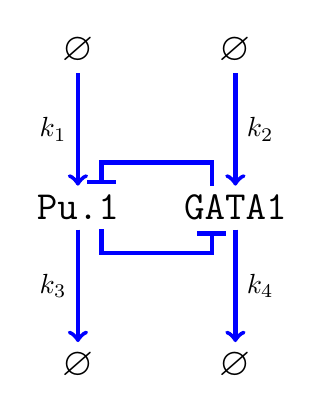
\begin{tikzpicture}[node distance=2cm]

\node (N0) {\Large $\varnothing$};
\node [right of = N0] (N1) {\Large $\varnothing$};
\node [below of = N0] (R0) {\Large \texttt{Pu.1}};
\node [below of = N1] (R1) {\Large \texttt{GATA1}};
\node [below of = R0] (N2) {\Large $\varnothing$};
\node [below of = R1] (N3) {\Large $\varnothing$};

\draw [->,ultra thick,blue] (N0) -- node[left, black] {$k_1$} (R0);
\draw [->,ultra thick,blue] (N1) -- node[right, black] {$k_2$} (R1);
\draw [->,ultra thick,blue] (R0) -- node[left, black] {$k_3$} (N2);
\draw [->,ultra thick,blue] (R1) -- node[right, black] {$k_4$} (N3);

\draw [-|,ultra thick,blue]
($ (R0) + (3mm,-2.75mm) $)
-- +(0,-3mm) %node[below, black] {$v_3$}
-| ($ (R1) - (3mm,3mm) $) ;

\draw [-|,ultra thick,blue]
($ (R1) + (-3mm,2.75mm) $)
-- +(0,3mm) %node[above, black] {$v_3$}
-| ($ (R0) - (-3mm,-3mm) $);

\end{tikzpicture}
\end{center}

There are four possible reactions happening within our model: $k_1$, $k_2$, $k_3$ and $k_4$. In our simulation, each reaction was assigned propensity value which roughly is proportional to the likelihood of the reaction happening in a given time:

$$P(R_i = k_l) \propto P_l$$

The propensity $P$ of decay reactions $k_3$ and $k_4$ roughly follows the mass action law of chemical reaction:

$$P_l = k_l \cdot A {;} \; l \in [3, 4]$$

For production reactions $k_1$ and $k_2$ we assume Michaeli-Menten inhibition kinetics that influences the production of the species. In this assumption, the inhibiting characteristics of a species on another species negatively influences the creation rate of the species it inhibits. The propensity of the reactions are thus,

$$P_1 = k_1 \cdot \frac{\texttt{GATA1}^{-n}}{\texttt{GATA1}^{-n} + K_{P1}^{-n}}$$

$$P_2 = k_2 \cdot \frac{\texttt{Pu.1}^{-n}}{\texttt{Pu.1}^{-n} + K_{P2}^{-n}}$$

\section{Bla}

\end{document}
